%! Author = charon
%! Date = 1/22/24

\section{Fuzzing-Kampagne}\label{sec: fuzzing-kampagne}
Eine Fuzzing-Kampagne folgt einer in der Regel festen Struktur.
\begin{figure}[h]
    \frame{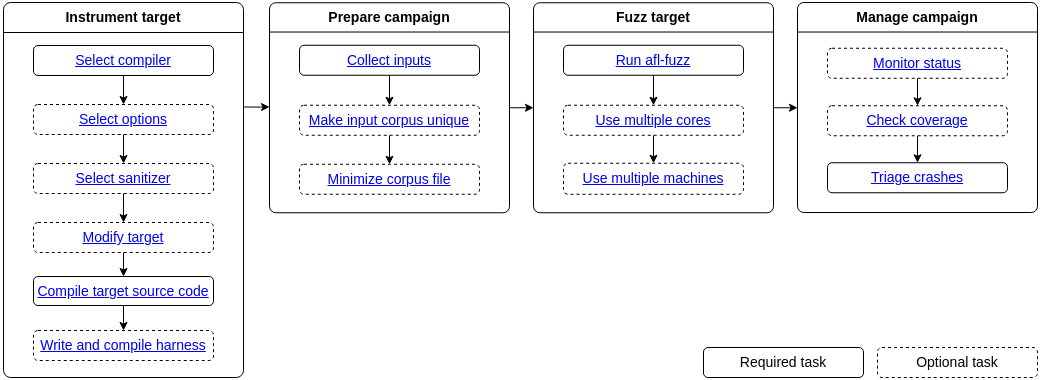
\includegraphics[width=\linewidth]{img/fuzzing-process-overview}}
    \caption{Visuelle Darstellung einer Fuzzing-Kampagne in mehreren Etappen, wenn der Quellcode eines Programms zur Verfügung steht~\cite{fuzzing-process-image}.}\label{fig:fuzzing-zyklus}
\end{figure}\\
Der erste Schritt besteht darin, das zu untersuchende Programm zu instrumentieren.
Wenn der Quellcode der Applikation verfügbar ist, können in diesem Schritt Anpassungen am Quellcode gemacht werden.
Dies geschieht, indem von~\gls{afl} bereitgestellte Funktionen und Makros in den Code geschrieben werden.
Dadurch ist es möglich, den Teil der Applikation zu isolieren, der untersucht werden soll.\\
\linebreak
Als Nächstes kommt die Sammlung möglicher Inputs für das instrumentierte Programm.
Hierbei werden alle gültigen Eingaben gesammelt.
Dabei ist zu beachten, dass die Dateien, die die Eingaben beinhalten, möglichst klein gehalten werden.
Um möglichst wenig Zeit und Performance der Kampagne zu verlieren, sollte mit dem von~\gls{afl} bereitgestellten Werkzeug
\texttt{afl-cmin} sichergestellt werden, dass jede Eingabe für das Ablaufen eines anderen Codepfades verantwortlich ist.\\
\linebreak
Im Anschluss wird der Fuzzer gestartet und das Programm wird mit dem gelieferten Input getestet.
Der Fuzzer mutiert den Input, nachdem alle Testfälle bereits mindestens ein Mal mit dem zu untersuchenden Programm
geprüft wurden.
Es wird empfohlen, dass die Mindestdauer einer Kampagne mindestens eine Stage beträgt.
Eine Stage ist der Durchlauf der Kampagne, bis keine neuen Codepfade mehr entdeckt werden.
Die benötigte Zeit für das Durchlaufen einer Stage hängt von der Komplexität des Programms ab.
Sie kann von einem Tag bis zu einer Woche dauern.\\
\linebreak
Zuletzt werden die gefundenen Abstürze und Hänger -- sofern sie gefunden wurden -- untersucht und verifiziert.\\
Beim Fuzzing ohne Sourcecode fällt jedoch der Schritt der Instrumentierung weg.
Dieser Schritt wird von dem~\gls{qemu} Modus des Fuzzers übernommen.\\
\linebreak
Eine solche Kampagne stellt einen zyklischen Prozess dar.
Nachdem eine Kampagne abgeschlossen wurde, ist es ratsam die bereits gefundenen Daten im Output-Verzeichnis wiederzuverwenden
und beim Schritt der Vorbereitung der Kampagne von vorne anzufangen.
%! Author = charon
%! Date = 2/8/24
\subsection{Instrumentation des Programms mit AFL++}\label{subsec: binary-only-instrumentation}
Fuzzing mit~\gls{afl} folgt einer klaren Vorgehensweise.
Da es sich bei der Umsetzung der Fuzzing Kampagne um ein Closed-Source-Binary handelt, wird der von ~\gls{afl}
bereitgestellte~\gls{qemu} verwendet.
\gls{qemu} ist eine Virtualisierungsumgebung, welche dafür verwendet wird, das Binary in einer emulierten
Umgebung starten zu können.
Aufgrund der hohen flexibilität von~\gls{qemu} ist es auch möglich, plattformunabhängig Binarys einer anderen Architektur auszuführen.
Somit ist es möglich, auf einer~\gls{arm} Plattform Programme mit x86 Architektur und umgekehrt auszuführen.
Die Plattformunterstützung muss beim Bau von~\gls{afl} manuell mitgegeben werden.
Das kann durch das Bauen des~\gls{qemu}-Supports mithilfe des Komfortscripts \textit{build\_qemu\_support.sh} in Kombination des
Setzens einer Umgebungsvariable \texttt{CPU\_TARGET=arm}~\ref{lst:build-qemu} erreicht werden~\cite{afl-build-qemu}. \\
Dieser Modus ist beim Starten des Fuzzers mithilfe des \texttt{-Q} Flags benutzbar.
Wie die~\gls{qemu} Umgebung mit der Firmware vorbereitet wird, ist in Abschnitt~\ref{subsec: bwrap} beschrieben.

%! Author = charon
%! Date = 2/8/24

\subsection{Übergabe von Daten als Parameter mithilfe von LD\_PRELOAD}\label{subsec: desocketing}
Wie bereits in Abschnitt~\ref{subsubsec:fuzzing-netzwerk-app} erläutert, ist das Fuzzen einer Netzwerkapplikation in dem bereits
implementierten Featureset von \gls{afl} nicht enthalten.
Hierzu kann eine Bibliothek selbst implementiert und als shared object kompiliert werden, sodass diese zum Start
der Applikation, mithilfe einer Umgebungsvariable namens \texttt{LD\_PRELOAD}, in die Applikation geladen wird.
Die Bibliothek beinhaltet eine eigene Implementierung der Syscalls \texttt{accept()}, \texttt{recv()}, \texttt{send()}
und \texttt{socket()}, welche die Funktionalität der bereits in libc-Bibliothek enthaltenen Funktionen überschreibt.
Um diese Funktionen effektiv für \gls{afl} nutzen zu können, müssen die genannten Syscalls so umgeschrieben werden, dass
Input, welcher über einen Netzwerksocket empfangen werden würde, stattdessen über die Eingabe von Dateien als Startparameter
übergeben wird.
Dieser Vorgang wird in der Fuzzing Community auch \textit{desocketing}~\cite{desocketing} genannt.
\gls{afl} besitzt bereits die Funktionalität ein shared object in Form einer \textit{.so} Datei in das zu untersuchende
Programm zu laden.
Unter \gls{afl} wird die Umgebungsvariable \texttt{AFL\_PRELOAD} genannt.\\
Bei diesem Binary werden jedoch keine Standard-Syscalls verwendet, sondern eine vom Hersteller implementierte Abstraktionsschicht,
welche die Funktionalität der Syscalls erweitert.
\begin{figure}[h]
    \frame{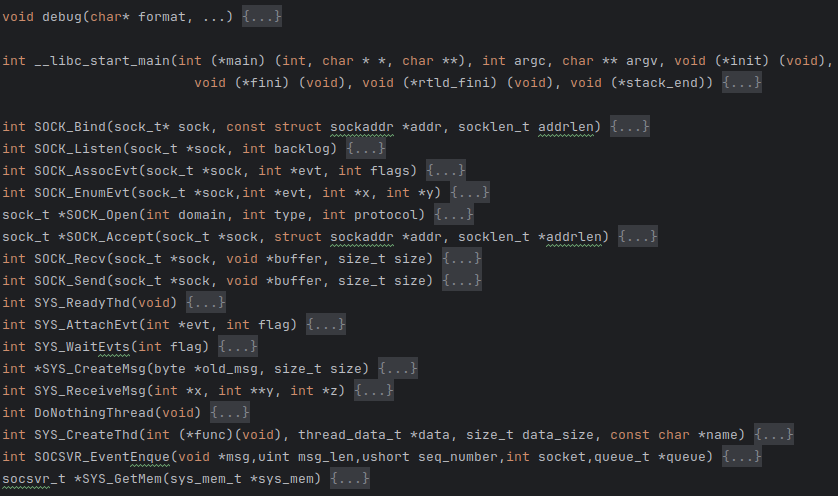
\includegraphics[width=\linewidth]{img/overwritten-funcs}}
    \caption{Zeigt die von Pahl überschriebenen Funktionen der preload Bibloiothek sockfuzz.so.
            Sie bestehen aus der vom Hersteller implementierten Abstraktionen der Standardfunktionen
            der libc Bibliothek.}\label{fig:overwritten-funcs}
\end{figure}\\
Das Ziel der Bibliothek ist es, das Überschreiben des \gls{tcp}-Sockets auf Port 7142, auf dem der gewünschte Netzwerkservice
läuft, sodass beim Fuzzen der Applikation keine Netzwerkanfragen lokal simuliert werden müssen.
Wichtig zu erwähnen ist hierbei, dass das direkte Senden von Daten an das Programm über das C \gls{cli} eine Performancesteigerung
um den Faktor der Größe 10 entspricht~\cite{afl-best-practice}.
Dies ist darauf zurückzuführen, dass weniger Overhead über den \gls{tcp}-Stack mitgegeben werden muss.
Ausschlaggebend bei dem Überschreiben der Abstraktionsschicht sind alle Funktionen, die nach einem Socket verlangen, sowie
die Funktion \texttt{\_\_libc\_start\_main()}.\\
Die Funktion \texttt{\_\_libc\_start\_main()}~\cite{libc-start-main} ist der Einstiegspunkt eines ausführbaren C-Programms und sorgt für das Initialisieren
der Laufzeitumgebung des Programms.
Ebenfalls ist die Funktion dafür verantwortlich die \texttt{main()} Funktion mit den zum Starten des Programms benötigten
Parametern (typischerweise \texttt{int argc} und \texttt{char *argv[]}) aufzurufen.\\
Der Einsprungspunkt muss überschrieben werden, damit die von \gls{afl} generierten Eingaben an das Programm als
Parameter zum Start des Programms übergeben werden können.
Dazu wird der \texttt{char *argv[]} Parameter der \texttt{main()} Funktion betrachtet.
Da der erste übergebene Parameter in C immer das Programm selbst ist, ist der zweite Parameter \texttt{argv[1]} der ausschlaggebende
Parameter.
Dieser über die Konsole übergebene Parameter wird bisher nicht von dem Programm verwendet und kann somit zur Übergabe der
Eingaben verwendet werden.
Als Nächstes wird die übergebene Datei an das Programm weitergegeben und gelangt weiter in den Calltree.
\gls{tcp}-Sockets unter auf \gls{unix} basierten Systemen arbeiten mit (Pseudo-)Dateien, welche einen Datenstrom repräsentieren.
Somit müssen alle Syscalls, welche auf den Socket 7142 verweisen, angepasst werden.
Sie sollen nicht mehr auf eine Datei, welche einen Socket repräsentiert, sondern auf die Datei, die von \gls{afl}
erzeugt wird, zugreifen.
Dafür soll die abstrahierte Version \texttt{SOCK\_Bind()} des \texttt{bind()} Syscalls überschrieben werden.
Er ist dafür verantwortlich, dass die Kommunikation über den richtigen Socket erfolgt.

%! Author = charon
%! Date = 2/8/24

\subsection{Optimierungen}\label{subsec: optimierung}
Aufgrund der langsamen Durchführung eines Fuzzing-Zyklus, muss die Kampagne angepasst werden.
Je öfter ein Zyklus durchlaufen wird, desto höher ist die chance innerhalb eines Zeitintervalls Fehler im Programm zu finden.
Ein Zyklus besteht aus dem Starten der Applikation, Weiterreichen der Daten bis zur gewünschten Stelle, der Terminierung
des Programms und Mutation des Inputs anhand des erlangten Feedbacks.\\
Ein Schritt zur Beschleunigung der Kampagne wäre, den Netzwerkservice der Applikation mittels Reverse-Engineering-Techniken
zu isolieren.
Dieser Prozess ist jedoch sehr zeitintensiv und zum Zeitpunkt der Verfassung dieser Arbeit nicht umsetzbar.
\subsubsection{Minimierung des Korpus}
Ein wichtiger Bestandteil einer erfolgreichen Fuzzing-Kampagne ist der Korpus.
Er ist das Mittel, mit dem \gls{afl} neue Codepfade (bzw.\ Call-trees) durchlaufen kann.
Ein Korpus ist nur dann einzigartig, wenn alle darin enthaltenen Daten jeweils unterschiedliche Codepfade ablaufen und eine möglichst
große Tiefe -- also möglichst viele branch edges -- im Code erreichen.
Für den ersten test des Fuzzers werden alle dokumentierten Funktionen verwendet und getestet.
Die Funktionen haben jeweils anders implementierte Handler für ihren speziellen Anwendungsfall.
Zum Prüfen, ob es redundanten Input gibt, empfiehlt es sich, die Umgebungsvariable \texttt{AFL\_DEBUG=1} zu setzen.
Sie ermöglicht es, weitere Informationen, wie Debug-Instruktionen des Programms (alle print-Statements und alle \texttt{puts()} aufrufe)
oder Informationen zur aktuell laufenden Kampagne anzuzeigen.
\begin{figure}[h]
    \frame{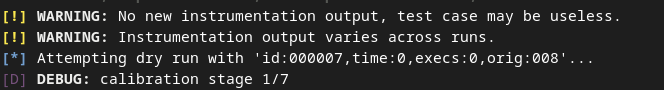
\includegraphics[width=\linewidth]{img/unique-corpus}}
    \caption{Zeigt eine Warnung von \gls{afl}.
    Sie warnt vor einem oder mehrerer Testcases, welche duplizierte Codepfadabdeckung
    bezwecken.}\label{fig:unique-corpus}
\end{figure}\\
\gls{afl} bietet ein Tool namens \texttt{afl-cmin}~\cite{afl-cmin} zum Minimieren der Testcases und zum Prüfen des Korpus.
Das Tool folgt einer ähnlichen Syntax wie \texttt{afl-fuzz} (siehe Listing: \ref{lst:afl-synthax}), wobei das Flag \texttt{-i} für den Ordner mit dem Korpus steht,
der analysiert werden soll.
Das Flag \texttt{-o} steht für den Ordner, in den der minimierte Korpus geschrieben werden soll.
Die Verwendung des Tools hat den Vorteil, dass das Fuzzing und die Mutation des Inputs nach jeder Stage eines Fuzzing-Zyklus,
aufgrund geringen Inputs, welcher mutiert werden muss und geringeren Inputs, welcher getestet werden muss, beschleunigt wird.
\subsubsection{Verwendung des Persistent Modes}\label{subsubsec:persistent-mode}
Als nächsten Performanceboost empfiehlt es sich, den bereits von \gls{afl} implementierten \textit{Persistent Mode} zu verwenden.
Der Persistent Mode erlaubt es \gls{afl}, ein Programm innerhalb zweier Speicheradressen mehrmals zu fuzzen, ohne dass der Prozess,
auf dem der Fuzzer läuft, erneut geforkt wird.
Hierzu muss das zu fuzzende Programm mit einem Hilfsprogramm wie dem \gls{gdb} des \gls{gnu}-Projekts untersucht werden,
um eine geeignete Speicheradresse als Einsprungspunkt definieren zu können.\\
Hierzu wird exemplarisch eine selbst entwickelte Applikation~\cite{example-tcp-server} zu Demonstrationszwecken hergenommen
und analysiert, welche ebenfalls einen \gls{tcp}-Stack verwendet.
Diese Applikation ist stark vereinfacht und bringt nicht die gleiche umfangreiche Funktionalität und Komplexität, wie das Ursprungsbinary
\textit{mmapp}, mit sich.
Um sich der Analyse eines \gls{arm}-Binarys anzunähern, wurde das Beispielsbinary für \gls{arm} kompiliert.
Dazu wurde ein Komfortskript~\cite{compile-script} geschrieben, welches einen bereits für diesen Zweck gebauten Docker-Container~\cite{docker-gcc} verwendet, um
das Binary zu kompilieren.
Die Besonderheit bei der Kompilierung des Binarys, um möglichst wenig Abweichung zu haben, ist die von dem Ursprungsbinary
\textit{mmapp} verwendete \gls{gcc} Version \textit{4.8.1}.
\begin{figure}[h]
    \frame{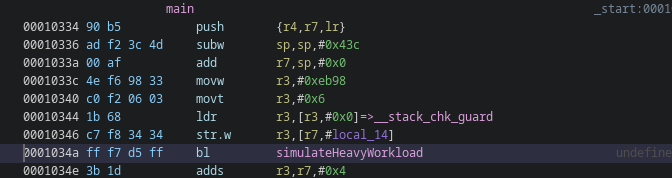
\includegraphics[width=\linewidth]{img/example-server-disassembly}}
    \caption{Zeigt den disassemblierten Code des selbst implementerten \gls{tcp}-Servers.
    In der Abbildung ist eine Funktion \texttt{simulateHeavyWorkload} in der Speicheradresse \texttt{0x001034a} zu sehen.
    Das Ziel der Definitiion der Startadresse ist es, diese zeitintensive Funktion zu umgehen.}\label{fig:example-server-disassembly}
\end{figure}\\
In Abbildung~\ref{fig:example-server-disassembly} ist der dazugehörige Disassembly Code des Beispielprogramms.
Hier ist zu sehen, dass die \texttt{main()} Funktion einen Funktionsaufruf auf eine Funktion namens \\ \texttt{simulateHeavyWorkload()}
macht.
Diese Funktion ist im übertragenen Sinne für das Initialisieren des \gls{iot}-Geräts verantwortlich.
Diese Funktion sollte während des Fuzzens möglichst nur ein Mal aufgerufen werden, da das Initialisieren der gesamten Peripherie
viel Zeit in Anspruch nimmt.
Das kann erzielt werden, indem man \gls{afl} mittels eines \textit{"persistent loop"}s innerhalb zweier Speicheradressen
instrumentiert.
Hierfür muss eine Startadresse \texttt{AFL\_QEMU\_PERSISTENT\_ADDR} an der gewünschten Speicheradresse \texttt{0x0001034e},
an der der Persistent-Loop anfangen soll, definiert werden.
Da hier nur ein Teil der \texttt{main()} Funktion gefuzzt werden soll und das Programm nicht unter normalen Bedingungen terminieren
sollte, muss eine Schlussadresse \texttt{AFL\_QEMU\_PERSISTENT\_RET}~\cite{qemu-persistent} definiert werden.
In diesem Fall soll der Persistent-Loop nach der Verarbeitung der empfangenen Daten enden. \\
\begin{figure}[h]
    \frame{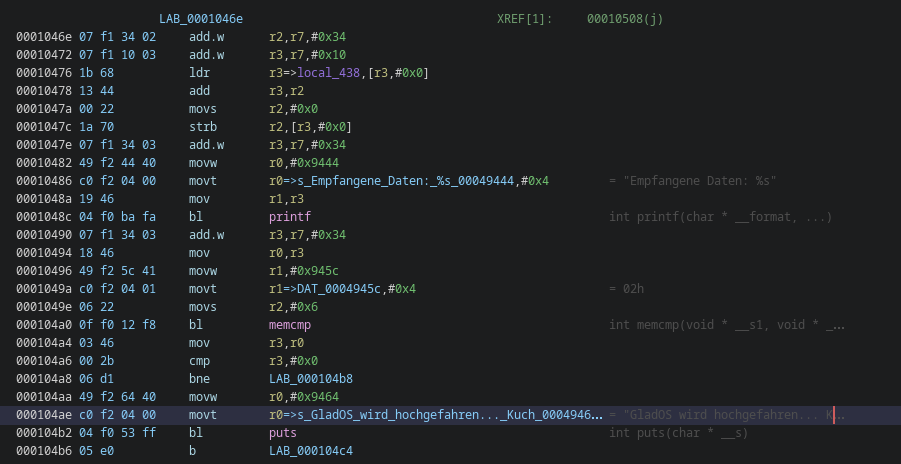
\includegraphics[width=\linewidth]{img/example-server-disassembly-end}}
    \caption{Disassembly des selbst implementierten \gls{tcp}-Servers. Diese Abbildung zeigt die für das Fuzzing wichtige
    Logik, in der die empfangenen Daten verarbeitet werden.
    Hierbei ist die Schlussadresse \texttt{0x000104ae} ausschlaggebend, in der die Verarbeitung der empfangenen
    Daten stattfindet.}\label{fig:example-server-disassembly-return}
\end{figure}\\
Die letzte Instruktion, die ausgeführt werden soll ist somit in der Speicheradresse \texttt{0x000104ae}~\ref{fig:example-server-disassembly-return}.
\subsubsection{Verwendung mehrerer CPU-Kerne}
Mit \gls{afl} ist es auch möglich, mehrere Instanzen des Fuzzers laufen zu lassen, um die Performance weiter zu verbessern.
Dazu wurde eine Funktionalität implementiert, die es mehreren Instanzen ermöglicht, parallel zueinander zu fuzzen.
Die Limitation besteht darin, dass nicht mehr Instanzen gestartet werden können, als \gls{cpu}-Kerne auf dem System verfügbar
sind.
Außerdem ist es ratsam, die Anzahl der Kerne zu untersuchen, die zur Verwendung einer Kampagne nützlich sind ohne einen
Perfomanceverlust zu bezwecken.
Diese Zahl liegt in der Regel zwischen 32 und 64 Kernen~\cite{afl-multiple-cores}.\\
\linebreak
Das Feature ist mit dem Setzen zweier Flags umsetzbar.
Under Verwendung des Flags \texttt{-M} kann die Hauptinstanz definiert werden.
Der Zweck eines Hauptfuzzers ist das Sammeln aller Testcases.
Dadurch werden nach der Terminierung einer Fuzzer-Instanz die gefundenen einzigartigen Testcases in den Hauptfuzzer importiert.\\
Jeder Untergeordnete Fuzzer wird mit dem \texttt{-S} Flag deklariert.\\
Dadurch entsteht die daraus resultierende Syntax zum Starten mehrerer Instanzen:
%! Author = chaorn
%! Date = 10.03.24

\begin{lstlisting}[language=bash, caption={Syntax des AFL fuzzing Befehls mit der Definition der
                    Hauptinstanz mithilfe des \texttt{-M} Flags},label={lst:multiple-cores-main}]
$ afl-fuzz -Q -M main -i in/ -o out/ -- /app/mmapp @@
\end{lstlisting}
%! Author = chaorn
%! Date = 10.03.24


\begin{lstlisting}[language=bash, caption={Syntax des AFL fuzzing Befehls mit der Definition einer
Nebeninstanz mithilfe des \texttt{-S} Flags},label={lst:multiple-cores-second}]
$ afl-fuzz -Q -S qasan -i in/ -o out/ -- /app/mmapp @@
\end{lstlisting}
Das Fuzzing mittels mehrerer Kerne macht am meisten Sinn, wenn jede Instanz eine andere Strategie umsetzt.
Es wird dabei empfohlen, andere Mutationsstrategien des Fuzzers zu verwenden, um möglichst viele mutierte Eingaben zu
erzielen, die voneinander abweichen.

